\documentclass[aspectratio=169]{beamer}
\usepackage{fontspec}
\setmainfont{Times New Roman}
\setsansfont{Arial}
\usepackage[vietnamese]{babel}
\usepackage{graphicx}
\title{FIT4013 -- Đề tài 16}
\subtitle{Dự đoán nguy cơ giao trễ -- kết quả tập con thực tế}
\author{Nhóm tự bổ sung thông tin thành viên}
\date{2026--2027}
\begin{document}
\frame{\titlepage}
\begin{frame}{Bài toán và dữ liệu}
Dự đoán sau khi tạo đơn, trước khi có kết quả giao. Target lớp 1: giao trễ.\\
DataCo thật: 180519 dòng, 53 cột, 65752 đơn. Đơn vị quan sát: dòng hàng.\\
Lớp 0 gồm cả đơn hủy: không diễn giải tất cả là giao đúng hạn.
\end{frame}
\begin{frame}{Chống leakage}
Bỏ Delivery Status, ngày giao thật, số ngày giao thật, Order Status, ID và thông tin cá nhân.\\
Group split theo Order Id: không cùng đơn ở train/test.\\
CV theo nhóm chỉ trên train. Test không chọn mô hình. Chưa phải đánh giá dự báo tương lai.
\end{frame}
\begin{frame}{Hai luồng, hai thuật toán}
A: median/mode, one-hot, scaling.\\
B: thêm tháng/thứ/giờ tạo đơn; giả thuyết lịch vận hành.\\
K-NN: k, metric, weights. Cây: depth, leaf, criterion.\\
Baseline cây mặc định và Dummy. Giới hạn 5999 dòng cùng subset/split cho mọi mô hình.
\end{frame}
\begin{frame}{Kết quả thật -- mô hình chọn bằng CV}
\resizebox{\textwidth}{!}{\begin{tabular}{lrrrrrr}
\hline
Model & Train F1 & CV F1 & Acc & Prec & Recall & F1 \\
\hline
baseline\_tree\_A & 0.999 & 0.669 & 0.653 & 0.699 & 0.623 & 0.659 \\
dummy\_A & 0.694 & 0.694 & 0.537 & 0.537 & 1.000 & 0.699 \\
knn\_A & 0.999 & 0.667 & 0.673 & 0.723 & 0.636 & 0.677 \\
tree\_A & 0.765 & 0.674 & 0.646 & 0.673 & 0.665 & 0.669 \\
knn\_B & 1.000 & 0.671 & 0.686 & 0.729 & 0.661 & 0.694 \\
tree\_B & 0.714 & 0.706 & 0.733 & 0.853 & 0.608 & 0.710 \\
\hline
\end{tabular}}\\
Cây B: Accuracy 0.7330, Precision 0.8533, Recall 0.6076, F1 0.7098.\\
Metric theo dòng; chưa có khoảng tin cậy hoặc xác suất hiệu chuẩn.
\end{frame}
\begin{frame}{Đánh giá theo đơn và phạm vi}
Gộp xác suất dòng bằng trung bình; ngưỡng cố định 0.5, mỗi đơn có trọng số bằng nhau.
\begin{center}
\begin{tabular}{lrrrr}
\hline
Mô hình & Accuracy & Precision & Recall & F1 \\
\hline
tree\_B & 0.7258 & 0.8554 & 0.6068 & 0.7100 \\
Dummy & 0.5532 & 0.5532 & 1.0000 & 0.7123 \\
\hline
\end{tabular}
\end{center}
Dummy dự đoán tất cả 423 đơn là trễ nên có Recall=1; F1 cao hơn một chút không đồng nghĩa hữu ích hơn.\\
Mẫu: 5999/180519 dòng (3.32\%), 2113/65752 đơn (3.21\%). Holdout lịch sử đã quan sát, không phải kiểm chứng độc lập mới.
\end{frame}
\begin{frame}{So sánh và overfitting}
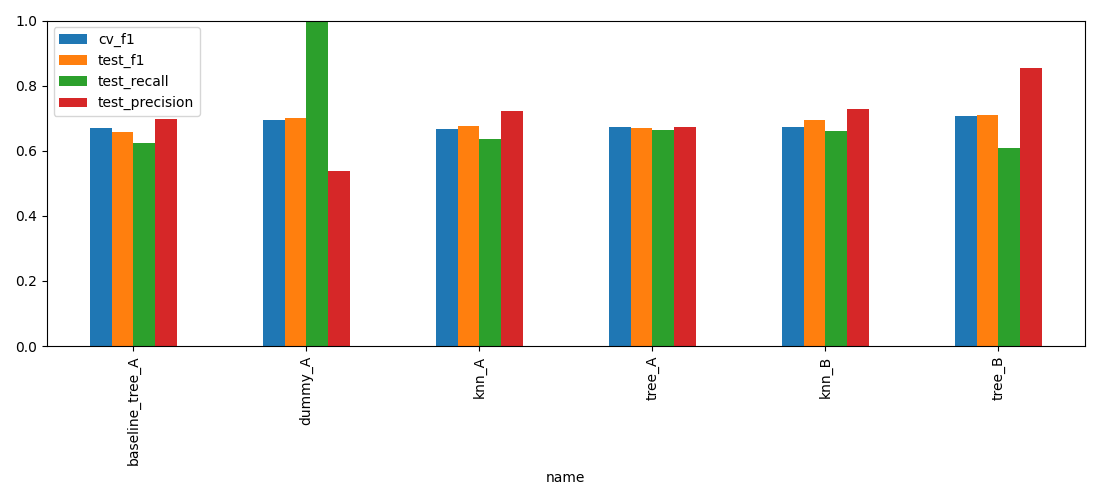
\includegraphics[width=.9\textwidth,height=.65\textheight,keepaspectratio]{../results/figures/comparison.png}
\end{frame}
\begin{frame}{Lỗi và hạn chế}
TN=478, FP=66, FN=248, TP=384.\\
Toàn bộ FN thuộc Standard Class; FNR nhóm 248/254.\\
Dummy Recall=1 nhưng cảnh báo tất cả đơn. Cây tăng precision, mất recall.\\
Chưa xác minh lợi ích kinh doanh; cần temporal validation, calibration và dữ liệu chi phí.
\end{frame}
\begin{frame}{Tái lập và liêm chính}
Chạy scripts/reproduce.ps1; xem manifest, hash, CV tables, tests và báo cáo.\\
AI được khai báo trong AI\_USAGE.md. Nhóm phải hiểu code, tự bổ sung đóng góp thật.\\
Bản nội dung chưa chuyển template học phần; không bảo đảm điểm số.\\
Nguồn: PDF FIT4013, Kaggle DataCo; nguồn gốc Mendeley DOI 10.17632/8gx2fvg2k6.5.
\end{frame}
\end{document}
